% 原始数据图保持不变；只覆盖图外的英文轴题与单位说明。
\begin{tikzpicture}
\node[anchor=south west,inner sep=0] (plot) at (0,0) {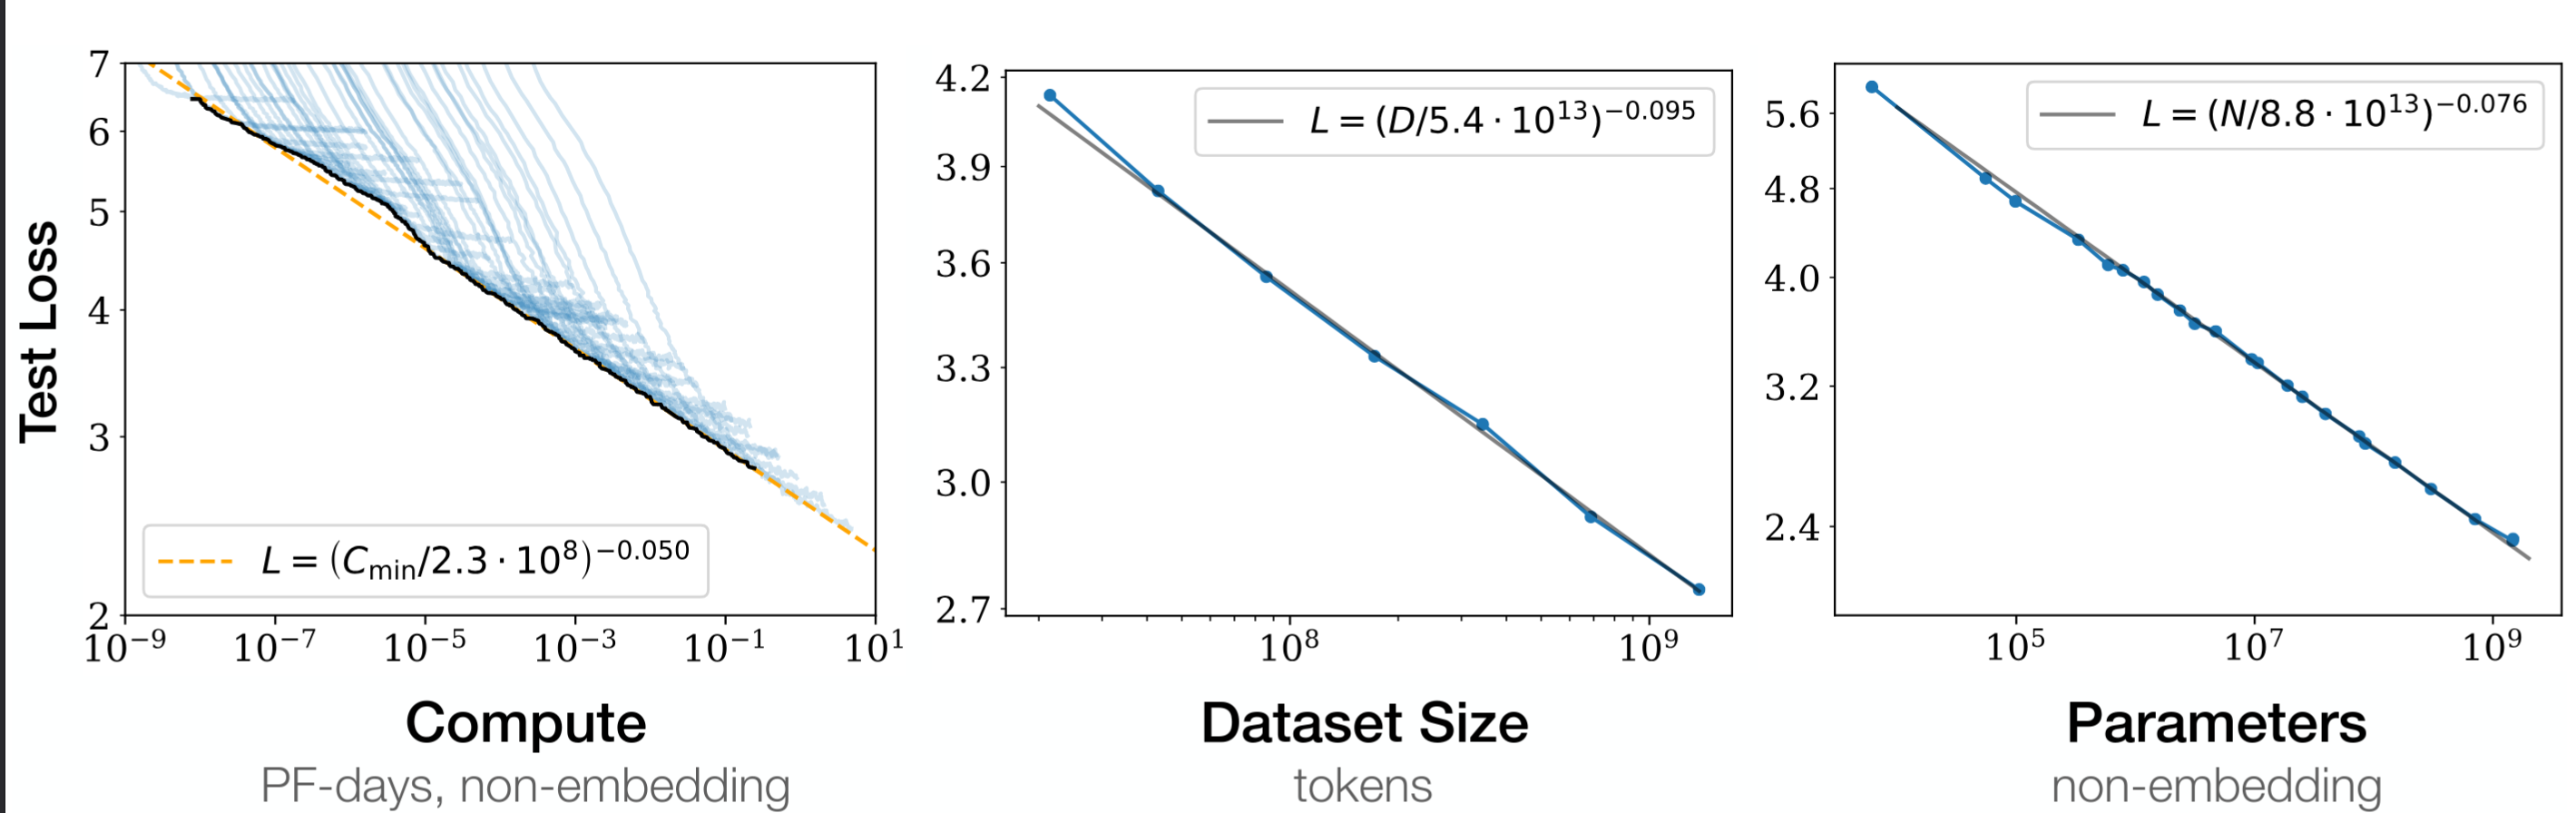
\includegraphics[width=.9\linewidth]{part1/visuals/scaling.png}};
\begin{scope}[x={(plot.south east)},y={(plot.north west)},every node/.style={font=\scriptsize,inner sep=0pt}]
\fill[white] (-.002,-.001) rectangle (.008,1.001);
\fill[white] (0,.20) rectangle (.035,.85);
\node[rotate=90] at (.015,.56) {测试损失};
\fill[white] (.045,0) rectangle (.995,.145);
\node at (.205,.108) {计算量};
\node at (.205,.025) {PF-days，不含嵌入参数};
\node at (.530,.108) {数据集规模};
\node at (.530,.025) {词元数};
\node at (.855,.108) {参数量};
\node at (.855,.025) {不含嵌入参数};
\end{scope}
\end{tikzpicture}
